
% JuliaCon proceedings template
\documentclass{juliacon}
\setcounter{page}{1}

\usepackage{hyperref}
\usepackage[linesnumbered,ruled,vlined]{algorithm2e}
\usepackage{graphicx}
\usepackage[font=small,labelfont=bf]{caption}
\usepackage{subcaption}
\usepackage{todonotes}

\setlength{\parindent}{2em}
\setlength{\parskip}{1em}

% Change link color
\hypersetup{colorlinks=true}

\begin{document}

% **************GENERATED FILE, DO NOT EDIT**************

\title{Solving Control Problems Using Differentiable Programming}

\author[1]{Tejan Karmali}
\author[2]{Neethu Mariya Joy}
%\author[2]{3rd author}
\affil[1]{National Insitute of Technology Goa, India}
\affil[2]{Birla Institute of Technology and Science Pilani, India}

\keywords{Julia, Differentiable Programming, Automatic Differentiation, Control Problems}



\maketitle

\begin{abstract}
In this paper we present a Differentiable Programming (DP) approach to solve problems which are currently tackled with reinforcement learning and other deep learning techniques. We discuss two major classes of problems - classical control problems and physical systems involving differential equations. The traditional approach to solving these problems is to use reinforcement learning. This paper proposes an alternate solution to these problems using differentiable programming. In addition to this approach we compare our method to the traditional solutions and showcase its clear advantages.

\headingtable

\end{abstract}

\let\thefootnote\relax\footnote{* Equal Contribution}

\section{Introduction}
\label{intro}

The success of deep learning is largely due to the idea of optimizing the weight parameters by differentiation. Wherever input and output are clearly defined, we can fit a model to approximate the function on it. Therefore, the pipeline is generally input-model-output, and is completely differentiable using any of the popular deep learning frameworks. The challenge is when we perform learning on a component that is programmatically non-differentiable using these frameworks.

The rise of Reinforcement Learning (RL) is because it can solve these non-differentiable blackboxes by only interacting with them. The algorithms of RL need not be problem specific. The downside here is that RL is

\begin{enumerate}
    \item sensitive to the hyperparameters
    \item slow to train
\end{enumerate}

In this paper, we explore the idea of differentiating through these so-called blackboxes, by leveraging the AD in julia\cite{bezanson2017julia}. In our experiments, we show differentiable programming was faster than RL as well as it used fewer hyperparameters. 

\section{Classic Control Problems}
\label{sec:ccprobs}
Control problems have a continuously operating dynamic system, which is controlled with a controller. There is a set of action defined for the controller, which may or may not change the state of the system. There is a score/reward defined for each state. Action has to be taken so as to maximise the cumulative score. Two of the classical control problems are Pole balancing problem and inverted pendulum problem. We describe the environments below.

\subsection{Pole Balancing}
\label{sec:cartpole}
In the this environment, a pole is attached to a cart. The cart moves on a one dimensional road. Initially the pole is upright and speed of the cart is 0. The goal is to balance the pole on the cart. State of the system is defined by 4 variables: position and velocity of the cart, and angular position and angular velocity of the pole. The action to be applied on the cart is to move it left or right by a constant speed. The positions of the cart and the pole are defined by equations of motion. These equations can be expressed as functions which are continuous. Therefore, a function can be defined which takes state $S_t$ as input and its output is state $S_{t+1}$. Reward at each timestep is 1 unit until the game is over. One episode of this environment consists of 200 timesteps at maximum. The problem is considered solved when mean cumulative reward across 100 episodes is greater than 195.\cite{Barto:1990:NAE:104134.104143, 1606.01540}

For differentiable programming pipeline, the reward should depend upon the model. That is, in the computation graph of the pipeline the reward node should have a connection with the model parameters. This is because we treat the problem as maximisation of cumulative reward, and consider the reward as negative of loss. Therefore, we define a custom reward. Ideal state of the system is that the pole should be upright and the cart should be at the centre. We use the product of difference of pole position and cart position from the ideal state as custom reward.

Since it has 2 discrete actions, we map them sign of the model output and define custom gradient for sign to pass the gradients through it unchanged.

\subsection{Inverted Pendulum}
\label{sec:pendulum}
In this environment, a pendulum needs to be balanced in inverted position. Action to be applied is a torque, whose value lies in a continuous space of $[-2, 2]$. State of the system is defined by the angular position and angular velocity of the pendulum. The reward depends on the state of the system and action applied. It is an unsolved environment, which means there is no specific reward limit above which is is considered solved.\cite{1606.01540}

Clamping the action value to lie between $[-2, 2]$ would mean gradients for all other values is 0. If initially model can generate values outside of this range, then learning will not take place. Hence, we modify this environment to accept action values across $[-\infty, \infty]$.
\subsection{Training Methodology}
\label{sec:training}
Since the we have to maximise the cumulative reward, we treat it the negative of that as loss function. Backpropagating the gradients obtained through this loss, we use the idea of backpropagation through time (BPTT). The gradients are backpropagated through the sequence of timeframes of an episodes. As the timeframes in an episode increase, it could be expensive to backpropagate through all of them. Hence we use truncated BPTT. We divide the sequence of timeframes in an episodes into small sequences of fixed length, and backpropagate through each one of them. In this way, the only hyperparameters we deal with are learning rate and those of the optimizer.


\begin{algorithm}[!htb]
    \caption{DP Algorithm to train agents}
    \label{alg:DiffRL}
    \SetAlgoLined
    \KwResult{Weights parameters to choose action for controller}\
    \While{not \textbf{game\_over(env)}}{
        gs = gradient(params(model)) \textbf{do}\\{
            loss = 0\;
            \For{i in 1 to SEQ\_LEN}{
                action = model(state(env))\;
                s$^\prime$, a, r, d = step!(env, action)\;
                loss += mean\_squared\_loss(r, MAX\_REWARD)\;
            }
            return loss\;
        }
        \textbf{end}\\
        \For{param in params(model)}{
            update!(optimizer, param, gs[param])\;
        }
    }
\end{algorithm}

\begin{figure}[!htb]
    \centering
    \begin{subfigure}[b]{0.4\textwidth}
        \centering
        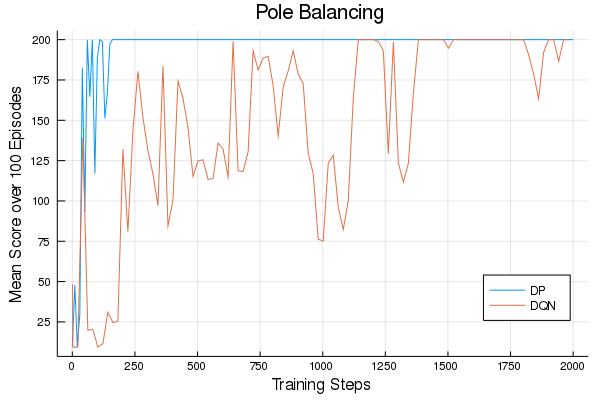
\includegraphics[width=\textwidth]{images/Agents/dp_vs_dqn.png}
        \caption{DP vs. DQN\cite{Mnih2015HumanlevelCT} on Pole Balancing task}
        \label{fig:score_plot_cartpole}
    \end{subfigure}
    
    \centering
    \begin{subfigure}[b]{0.4\textwidth}
        \centering
        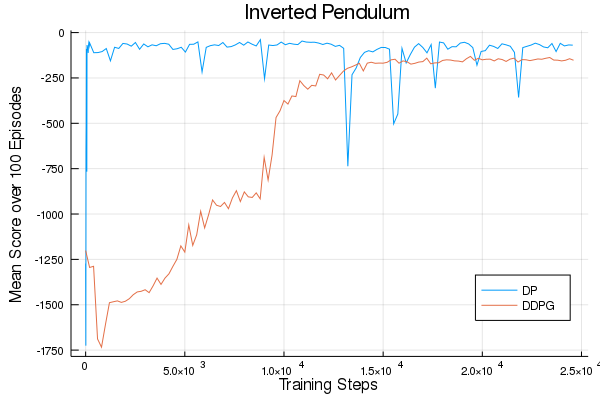
\includegraphics[width=\textwidth]{images/Agents/dp_vs_ddpg.png}
        \caption{DP vs. DDPG\cite{Lillicrap2015ContinuousCW} on Inverted Pendulum task}
        \label{fig:score_plot_pendulum}
    \end{subfigure}
    \caption{Comparison of DP with RL algorithms}
\end{figure}

\section{Differential Equations}
\label{sec:trebuchet}

Differential Equations are used to describe many natural phenomena. Problems in biological, chemical and physical systems can be expressed as ordinary differential equations or partial differential equations (\todo{ref: "Ordinary differential equations with applications in molecular biology" - Ilea, M., M. Turnea, and M. Rotariu .  }). There are a wide range of numerical integration methods available to solve these equations (\todo{ ref DiffrentialEquations.jl}). The sensitivity of the final state of an ODE solution with respect to the parameters of the ODE are of interest to many engineering applications. Flux is capable of calculating this by backpropagating through differential equation solvers (\todo{ ref https://arxiv.org/abs/1902.02376 ? }). Using these capabilities, we present a neural network training pipeline with an AD agnostic trebuchet simulator to aim at a target. The simulator is unaware of any parts of the AD system.

\subsection{Trebuchet}

% inside Trebuchet.jl

Unlike a simulation of a body in free-fall which can be simulated using one ODE, Trebuchet.jl(\todo{ ref Trebuchet.jl }) simulates shooting a projectile from a trebuchet by solving three ODEs, one after another. The three ODEs correspond to the stages when the projectile is on the ground, hanging on the sling, and released from the sling (\todo{ref virtualtrebuchet.com }). The transition between these stages and the termination involve root finders on the ODE solutions. We make use of Euler solver method with a constant time step to solve the ODEs and find the trajectory of the projectile. 

We are interested in creating a model that provides us with the right trebuchet parameters such as mass of the counter-weight and release angle, given any wind speed and target landing position. Here, we are not doing parameter estimation for a particular target but creating a model to find the parameters for any given target. We do so by constructing our loss value out of a fully differentiable chain containing the simulator. Our neural network takes the target position and the wind speed as inputs and produces the required trebuchet parameters as outputs. We then feed these values to the simulator which solves the ODEs to find the landing position. The landing position is compared with the target to get a scalar loss value. We can differentiate through this flow using Flux. We use forward-mode differentiation to find the gradient of the loss with respect to the trebuchet parameters and back-propagate it through the neural network. Once we have the gradients, we use an optimizer such as Adam to adjust the weights in the neural network.

\begin{algorithm}[!htb]
    \caption{DP Algorithm for trebuchet}
    \label{alg:DiffRLTrebuchet}
    \SetAlgoLined
    \KwResult{parameters for model to aim the trebuchet}\
    \For{windspeed, target in data}{
        gs = gradient(params(model)) \textbf{do}\\{
            angle, weight = model(windspeed, target)\;
            distance = simulator(windspeed, angle, weight)\;
            loss = mean\_squared\_loss(distance, target)\;
        }
        \textbf{end}\\
        \For{param in params(model)}{
            update!(optimizer, param, gs[param])\;
        }
    }
\end{algorithm}

\todo{Add the ODE Equations}

\section{Challenges}
We have used reward in loss function. The downside here is that reward has to be dependent on the model in the computation graph. If there is reward for time spent in the environment, or point scored against the opponent (sparse reward) then DP cannot capture that information. \\
Secondly, this approach needs to be generalised for environments with discrete actions. In Pole Balancing, we could map the action generated by the model from real domain to ${-1, 1}$ because the definition of action in pole balancing allowed to do so.

\section{Conclusion}
In conclusion, we have presented how julia can be leveraged to build differentiable systems. Integrating them with the machine learning pipeline can make an end-to-end differentiable pipeline. Using this pipeline we can define differentiable programming algorithm on it to solve the problem. We gave examples of how coupling differentiable control environments, and ODE solvers with neural networks can solve the problems in a novel and faster way.

\bibliographystyle{juliacon}
\bibliography{ref}

\end{document}

% Inspired by the International Journal of Computer Applications template
